\subsection{Компилятор} \label{sub111}

Компилятор~--- это программа, которая  принимает текст, написанный на~одном языке~--- \textit{исходном}, и~транслирует (переводит) его в~эквивалентный текст на~другом языке~--- \textit{целевом}~\cite{Aho2003}. Процесс компиляции можно разделить на~две части.

 Первая часть~--- \textit{анализ} (выполняется в несколько фаз) разбивает исходную программу на~составные части и~накладывает на~них грамматическую структуру. Затем эта структура используется для генерации промежуточного представления программы. Анализатор сообщает пользователю об~ошибках, собирает информацию об~исходной программе и~сохраняет в~\textit{таблицу символов}. Таблица символов~--- это структура данных, которая используются компилятором для хранения информации о~конструкциях исходной программы. Информация накапливается инкрементно в~фазе анализа компилятора и~используется фазой синтеза для генерации целевого кода.

Вторая часть~--- \textit{синтез} (выполняется генератором кода), строит требуемую целевую программу на~основе промежуточного представления и~информации из~таблицы символов.

Анализ и синтез делятся на несколько шагов, которые представлены на~рис.~\ref{img:compiler-structure-2}.

\newpage

\begin{figure}[ht]
	\centering
	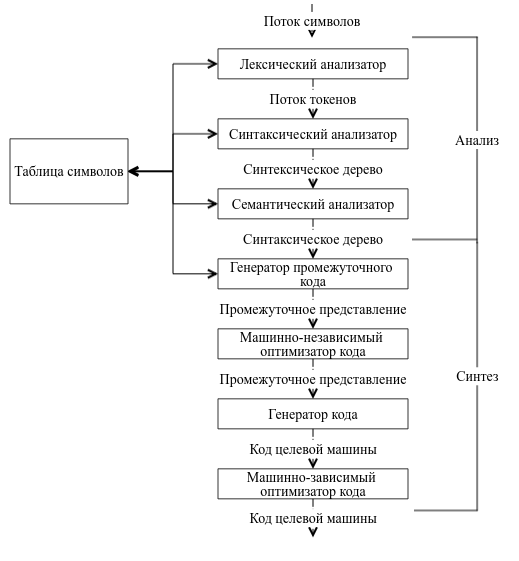
\includegraphics [scale=0.75] {compiler-structure}
	\caption{Схема взаимодействия фаз компилятора}
	\label{img:compiler-structure-2}
\end{figure}

Анализ:
\begin{itemize}
\item{\textit{Лексический анализ} или \textit{сканирование}. Лексический анализатор читает поток символов, составляющих исходную программу, группирует их в~значащие последовательности (лексемы), формирует для каждой лексемы специальные структуры данных, называемые токенами, и~передает их синтаксическому анализатору.}	
\item{\textit{Синтаксический анализ} или \textit{разбор}. Синтаксический анализатор использует информацию из предыдущей фазы и~на её основе строит синтаксическое дерево, в~котором каждый внутренний узел представляет операцию, а~дочерние узлы~--- аргументы этой операции.}	
\item{\textit{Семантический анализ}. Данная фаза компиляции использует синтаксическое дерево и~информацию из таблицы символов для проверки исходной программы на семантическую согласованность с~определением языка. Важной частью семантического анализа является проверка и~приведение типов.}
\end{itemize}

Синтез:
\begin{itemize}	
\item{\textit{Генерация промежуточного кода.} На этой фазе компилятор генерирует низкоуровневое промежуточное представление кода исходной программы, которое можно рассматривать как программу для абстрактной вычислительной машины.}	
\item{\textit{Машинно-независимая оптимизация кода.} Фаза машинно-независимой оптимизации кода пытается улучшить промежуточный код. Например, заменить вызов метода на~непосредственное выполнение тела метода в~месте вызова.}	
\item{\textit{Генерация кода.} В качестве исходных данных генератор кода получает промежуточное представление исходной программы и~отображает его в~целевой язык, как правило в~ассемблерный код.}
\item{\textit{Машинно-зависимая оптимизация кода.} Фаза машинно-зависимой оптимизации кода улучшает код целевой машины, учитывая особенности архитектуры процессора.}		
\end{itemize}


Процесс анализа компиляции разделен на~лексический, синтаксический и~семантический анализ по~ряду причин: 

\begin{enumerate} 
	\item{Упрощение разработки. Отделение лексического анализа от~синтаксического позволяет упростить как минимум одну из~фаз анализа. Например, удаление комментариев и~пробельных символов лексическим анализатором значительно проще, чем включение работы с~ними в~синтаксический анализатор.}
	\item{Увеличение переносимости компилятора. Например, для того, что~бы~компилятор работал на~разных операционных системах достаточно реализовать только часть генерации кода, вместо написания второго компилятора.}
	\item{Разделение зон ответственности. Каждый компонент отвечает только за определённую часть функциональности. Таким образом сокращается вероятность допущения ошибки, код каждого компонента становится легко модифицируемым. }
\end{enumerate}
